\documentclass[border=4pt]{standalone}
\usepackage{tikz}
\usetikzlibrary{arrows}
\begin{document}
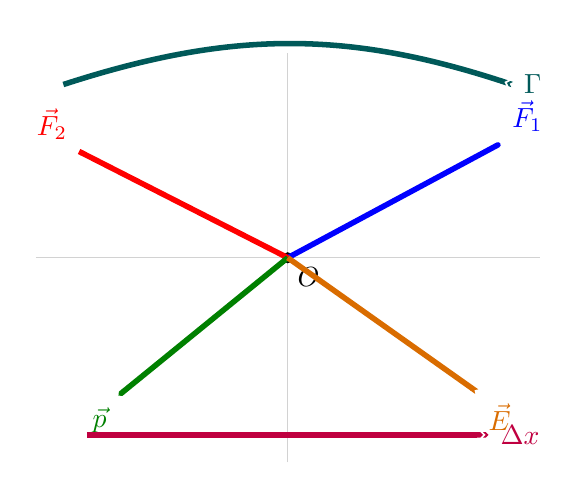
\begin{tikzpicture}
  \draw[gray!35] (-3.2,0) -- (3.2,0);
  \draw[gray!35] (0,-2.6) -- (0,2.6);
  \fill (0,0) circle (2pt) node[below right] {$O$};

  \draw[blue,line width=2pt,-{round cap}] (0,0) -- (2.7,1.45) node[above right] {$\vec F_1$};
  \draw[red,line width=2pt,-{butt cap}] (0,0) -- (-2.65,1.35) node[above left] {$\vec F_2$};
  \draw[green!50!black,line width=2pt,-{triangle 90 cap}] (0,0) -- (-2.15,-1.75) node[below left] {$\vec p$};
  \draw[orange!85!black,line width=2pt,-{triangle 90 cap reversed}] (0,0) -- (2.4,-1.7) node[below right] {$\vec E$};
  \draw[purple,line width=2pt,-{fast cap}] (-2.55,-2.25) -- (2.55,-2.25) node[right] {$\Delta x$};
  \draw[teal!70!black,line width=2pt,-{fast cap reversed}] (-2.85,2.2) to[bend left=18] (2.85,2.2) node[right] {$\Gamma$};
\end{tikzpicture}
\end{document}
